\documentclass[brazil,a4paper,11pt]{book}
\usepackage[T1]{fontenc}
\usepackage[utf8]{inputenc}
\usepackage{lmodern}
\usepackage[brazilian]{babel}
\usepackage{hyperref}
\usepackage{listings}
\usepackage{graphicx}

\begin{document}
\begin{titlepage}
  \begin{center}
  \textsc{{\small \textbf{Instituto de Matemática e Estatística da Universidade de São Paulo}}}
  \\[6cm]
  \textsc{{\large \textbf{Implementação do Método de Integração Numérica Runge-Kutta em GPGPU para Aplicações Científicas}}}
  \\[2cm]
  \textsc{Giancarlo Rigo\\
          Rafael Reggiani Manzo\\
          \textbf{Supervisor:} Prof. Doutor Marcel P. Jackowski}
  
  \vfill
  \today
  \end{center}
\end{titlepage}

\tableofcontents

\part{Objetiva}
\chapter{Introdução}

\section{Motivações}
O método de integração numérica de Runge-Kutta permite a aproximação da solução de problemas de valor inicial, podendo ser generalizado para a reconstrução de trajetórias tridimensionais a partir de campos vetoriais, que será o objeto desta monografia.

\section{Objetivos}
Como este método é computacionalmente custoso, porém altamente paralelizável, o primeiro objetivo é tê-lo implementado para \textit{GPU}, com \textit{CUDA} e \textit{OpenCL}, de forma que uma aplicação seja capaz de fazer sucessivas chamadas ao algoritmo e cada uma destas responda em um tempo curto o bastante para ser considerado em tempo real.

Com isto em mãos, fazer a mesma implementação em \textit{C++} para que possa ser feita uma comparação tanto com relação ao tempo gasto por cada chamada, quanto à corretude da implementação em \textit{GPU}. Assim, também, permitindo a implementação de uma visualização gráfica dos resultados com \textit{OpenGL}.

Por fim, quando alcançados estes objetivos, será possível implementar este algoritmo como um filtro para o \textit{VTK}, permitindo a implementação no software livre \textit{MedSquare}$^{\ref{medsquare}}$ da funcionalidade de tractografia em tempo real (\textit{real time fiber tracking}$^{\ref{fiber-tracking-article}}$).

\newpage
\section{Desafios}
Quando programamos para \textit{GPU} temos que ter em mente certas limitações da linguagem, como complexidade das estruturas de dados, a melhor forma de utilizar toda sua capacidade em paralelo, a forma mais eficiente de usar seus vários níveis de memória e, principalmente, como minimizar a transferência da \textit{RAM} para a \textit{GPU} e vice-versa. Caso contrário, muito provavelmente, a implementação em \textit{GPU} será mais lenta que uma para \textit{CPU}.

Ainda no contexto de programação para \textit{GPU}, um segundo desafio será a implementação em \textit{OpenCL} que é uma linguagem muito menos difundida que o \textit{CUDA} e ligeiramente diferente desta para implementar, pois permite que um mesmo código seja executado tanto em \textit{GPU} quanto \textit{CPU}.

Por fim, a implementação de um filtro para o \textit{VTK} torna a implementação do método ainda mais complexa pois ela deve se adaptar a sua arquitetura. Bem como, a adição de uma nova funcionalidade ao \textit{MedSquare}$^{\ref{medsquare}}$ pode exigir mais adaptações.

\chapter{Conceitos e tecnologias estudadas}

\section{Problemas de Valor Inicial}
São os problemas nos quais são dados:
\begin{itemize}
  \item um conjunto de pontos iniciais $P$;
  \item o valor de $f(P_{0})$ para cada $P_{0} \in P$;
  \item um sistema de uma ou mais equações diferenciais ordinárias (EDOs) em $f$;
  \item e um tamanho de passo $h$.
\end{itemize}

E desejamos obter $f(P_{0} + h)$.

\section{Método de Integração Numérica Runge-Kutta}\label{rungekutta}
É um dos métodos para resolução de Problemas de Valor Inicial através da obtenção de uma aproximação para o valor de $f(P_{0} + h)$. Ele é uma generalização do Método de Euler através da aplicação de séries de Taylor (\ref{numerical-recipes}). Essa generalização nos permite a obtenção de diversas ordens do método, dentre as quais as mais comuns são 2 e 4, conhecidos como \textit{RK2} (ou, também, \textit{método do ponto médio}) e \textit{RK4}.

Ambos os métodos possuem termos da ordem de uma potência de $h$. Estes termos são o erro associado ao método e, portanto, quanto menor o tamanho do passo, menor o erro do método.

Logo, dado um Problema de Valor Inicial conforme descrito acima com uma única equação diferencial $g = f'$, temos os seguintes métodos definidos para apenas um ponto inicial, embora sua generalização para mais pontos consista apenas de sucessivas aplicações do mesmo método para cada ponto.

  \newpage
  \subsection{Ordem 2}
  Sejam $k_{1}$ e $k_{2}$ variáveis auxiliares, temos a seguinte expressão para o método de ordem 2:
  \newline
  \newline
  $k_{1} = h\ldotp g(P_{0})$\\
  $k_{2} = h\ldotp g(P_{0} + \frac{k_{1}}{2})$\\
  $f(P_{0} + h) = f(P_{0}) + k_{2} + O(h^{3})$
  
  \subsection{Ordem 4}
  Sejam $k_{1}$, $k_{2}$, $k_{3}$ e $k_{4}$ variáveis auxiliares, temos a seguinte expressão para o método de ordem 4:
  \newline
  \newline
  $k_{1} = h\ldotp g(P_{0})$\\
  $k_{2} = h\ldotp g(P_{0} + \frac{k_{1}}{2})$\\
  $k_{3} = h\ldotp g(P_{0} + \frac{k_{2}}{2})$\\
  $k_{4} = h\ldotp g(P_{0} + k_{3})$\\
  $f(P_{0} + h) = f(P_{0}) + \frac{k_{1}}{6} + \frac{k_{2}}{3} + \frac{k_{3}}{3} + \frac{k_{4}}{6} + O(h^{5})$

\section{Campo vetorial como discretização de EDOs}
Se calcularmos o valor de cada EDO em um conjunto finito de pontos $P$ obteremos então um campo vetorial que pode ser compreendido como a discretização destas equações neste conjunto limitado.
  \subsection{Algoritmos de aproximação}\label{aproximacao}
  Porém esta discretização exige uma aproximação para o caso onde desejamos obter um o valor da equação, em um ponto não definido no campo vetorial.

  \label{exemplo-campo}Como, por exemplo, o caso onde as coordenadas de todos os pontos são inteiros e o ponto desejado possui alguma coordenada racional.

    \subsubsection{Nearest Neighbour}
    No caso do exemplo acima (\ref{exemplo-campo}), este algoritmo simplesmente aproxima o ponto desejado para o ponto mais próximo a este que esteja definido no campo vetorial.

    Ou seja, um algoritmo para uma das coordenadas cujo valor pretendido seja $a$, que pode ser generalizado para as demais, é:
    
    \begin{enumerate}
      \item Se $(a - \lfloor a\rfloor) \geq  0.5$ então devolvemos o valor em $\lceil a\rceil$;
      \item Caso contrário, então devolvemos o valor de $\lfloor a\rfloor$.
    \end{enumerate}
    
    \newpage
    \subsubsection{Interpolação trilinear}
    Antes de definir a interpolação trilinear é preciso definir a \textbf{interpolação linear}. Na qual dados dois pontos, $P_{1}$ e $P_{2}$, para os quais uma função $f$ está definida, o valor desta função em um ponto $P$, $f(P)$, sobre a reta $r$ que liga estes dois pontos é a ponderação do valor de $f(P_{1})$ e $f(P_{2})$ pela distância de $P$ a $P_{1}$ e $P_{2}$, respectivamente.
    
    Este método muito utilizado no $\Re ^{2}$ é dado por:
    
    $f(P) = f(P_{1}) + \frac{(f(P_{2}) - f(P_{1}))}{(P_{2} - P_{1})}\ldotp (P - P_{1})$
    
    Por sua vez a interpolação trilinear é inerentemente utilizada no $\Re ^{3}$. Ela pondera os oito pontos $P_{1}$, $P_{2}$, $P_{3}$, $P_{4}$, $P_{5}$, $P_{6}$, $P_{7}$ e $P_{8}$ definidos no campo para então obter $P$.
    
    No caso do exemplo \ref{exemplo-campo}, podemos compreender estes quatro pontos como os vértices do cubo que contém o ponto de interesse.
    
    \begin{figure}[!h]
      \begin{center}
         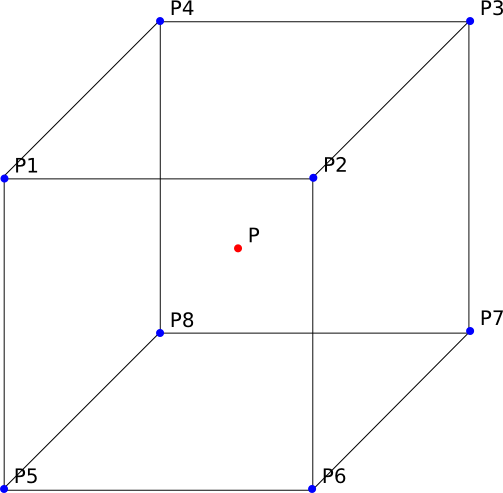
\includegraphics[width=60mm, height=60mm]{images/trilinearinterpolation.png}
         \label{fig:trilinearinterpolation}
         \caption{Os pontos cujas coordenadas são todas as combinações de chãos e tetos do ponto $P$ formam um cubo unitário que o contém}
      \end{center}
    \end{figure}
     
    A idéia do algoritmo é interpolar os pontos de cada aresta dois a dois na mesma coordenada sucessivamente. Se interpolarmos sobre $x$, depois sobre $y$ e por fim sobre $z$ para obtermos $P$, teremos as seguintes interpolações a serem calculadas:
    
    \begin{enumerate}
      \item $X_{1} = intp(P_{1}, P_{2})$;
      \item $X_{2} = intp(P_{3}, P_{4})$;
      \item $X_{3} = intp(P_{5}, P_{6})$;
      \item $X_{4} = intp(P_{7}, P_{8})$;
      \item $Y_{1} = intp(X_{1}, X_{2})$;
      \item $Y_{2} = intp(X_{3}, X_{4})$;
      \item $P = intp(Y_{1}, Y_{2})$.
    \end{enumerate}
    
    Onde $intp(A,B)$ é uma função que calcula a interpolação linear de $A$ e $B$.

\section{Computação de propósito geral na unidade de processamento gráfico}
\label{gpgpu}
Mais conhecida como \textit{General-Purpose computing on Graphics Processing Units (GPGPU)}, trata-se de  criar trechos de código que são executados na unidade de processamento gráfico ao invés de fazê-lo na \textit{CPU}. Este recurso é interessante para algoritmos altamente paralelizáveis uma vez que as unidades de processamento gráfico foram feitas para isto.

Por exemplo, uma NVIDIA GeForce GTX 690 possui mais de 3000 núcleos de processamento (\textit{CUDA Cores}) a aproximadamente 900MHz cada e 4GB de memória dedicada (\ref{gtx690}). O que representa um pequeno \textit{mainframe} à disposição para a execução de algoritmos paralelos. 

Ainda no princípio das placas gráficas dedicadas, percebendo seu poder computacional, teve início a programação de algoritmos gerais (isto é, algoritmos que não sejam de processamento gráfico) em termos de operações gráficas. Ou seja, os algoritmos eram traduzidos em termos multiplicações de matrizes para poderem ser processados na placa gráfica.

Com o crescimento deste tipo de uso, surgiu a linguagem \textit{Cg} facilitando a confecção de programas para a placa gráfica, mas que no fim das contas era compilado em termos de \textit{DirectX} ou \textit{OpenGL shaders}. Ou seja, ainda era apenas uma abstração para o processamento gráfico.

O que enfim levou a criação de linguagens de mais alto nível como \textit{OpenCL} e \textit{CUDA} que, do ponto de vista do programador, funcionam como uma extensão para linguagens como \textit{C}, \textit{C++}, \textit{Fortran} etc. Permitindo que quase não haja distinção entre programar para \textit{GPU} ou \textit{CPU}.

Antes de apresentar os detalhes das linguagens, é preciso destacar específicidades da programação para GPU que ainda não foram abstrataídos:

\begin{itemize}
  \item O trecho de código executado na \textit{GPU} é chamado de \textit{kernel}. Cada instância deste é chamada de \textit{thread}. Um conjunto de threads pode ser agrupado no que a NVIDIA chama de \textit{bloco}. E, por sua vez, estes podem ser agrupados no que a NVIDIA chama de \textit{grade};
  \item Os dados sobre os quais os algoritmos vão operar precisam ser transferidos da memória principal à memória dedicada da placa gráfica, através do barramento, e o resultado de volta. Esta transferência pode ser muito lenta, pois além do próprio barramento ser um gargalo, este ainda é compartilhado com todos os demais periféricos. Portanto, o primeiro objetivo é minimizar estas transferências a apenas o necessário e, quando elas forem necessárias, que sejam feitas em grandes quantidades de dados para usar toda a banda;
  \item Os diversos núcleos de processamento da unidade de processamento gráfico na verdade estão agrupados fisicamente agrupados no que é chamado de \textit{stream multiprocessors} pela NVIDIA. Isto é importante, pois todas as \textit{threads} de um bloco devem ser executadas no mesmo \textit{stream multiprocessor}. Ou seja, para utilizar toda capacidade da placa gráfica, é preciso ter vários \textit{blocos};
  \item A placa gráfica possui diferentes níveis de memória. A memória local contém as variáveis locais da thread, a memória compartilhada é a de acesso mais rápido para leitura, por estar dentro de cada \textit{stream multiprocessor}, e por fim a memória global. Para tornar o acesso à memória o menos custoso possível, é preciso fazer uso da memória compartilhada, embora o seu uso sem os devidos cuidados pode gerar erros de inconsistência semelhantes aos que podem ser vistos em um cache mal implementado. Ou seja, a escrita deve ser cuidadosa.
\end{itemize}
  \subsection{Linguagem CUDA}
  Atualmente na versão 4.2, é classificada como uma arquitetura para computação de propósito geral em paralelo introduzida em 2006 pela NVIDIA. Do ponto de vista do programador é uma extensão disponível para as linguagens \textit{C}, \textit{C++} e \textit{FORTRAN}. Os principais elementos do \textit{CUDA} são a hierarquia de agrupamento das threads, os níveis de memória e as barreiras de sincronização.
  
  A hierarquia de agrupamento consiste de dois níveis: grades (\textit{grids}) e blocos (\textit{blocks}). Um bloco agrupa muitas threads e uma grade, por sua vez, agrupa muitos blocos. Além de os blocos afetarem diretamente o escalonamento como descrito em \ref{gpgpu}, cada bloco possui um limite de threads que pode conter e o mesmo para grades com relação a blocos (este limite depende do hardware). Outro uso interessante para este agrupamento, é organizar processamento sobre dados que possuem três dimensões.
  
  O primeiro nível de memória é a memória local de cada thread privada, depois a memória compartilhada de cada bloco e, por fim, a memória global acessível por todas as threads. A memória global persiste até que seja desalocada pelo programa, enquanto as demais persistem apenas enquanto suas estruturas existem. As memórias local da thread e compartilhada do bloco são as mais rápidas ao custo de seu escopo reduzido.
    
  \subsection{Linguagem OpenCL}

\chapter{Atividades Realizadas}

\section{Representação do campo vetorial e das fibras em C++}
\section{Implementações dos Métodos Runge-Kutta, Nearest Neighbour e Interpolação Linear em C++}
\section{Implementações dos Métodos Runge-Kutta, Nearest Neighbour e Interpolação Linear em CUDA}
\section{Implementações dos Métodos Runge-Kutta, Nearest Neighbour e Interpolação Linear em OpenCL}
\section{Interface de Visualização dos Resultados em OpenGL}
\section{Integração com o MedSquare através do VTK}

\chapter{Resultados e produtos obtidos}

\section{Implementações dos métodos Runge-Kutta, Nearest Neighbour e Interpolação Trilinear}
  \subsection{Protótipo básico}
  O protótipo básico foi uma prova de conceito bem sucedida para a implementação do método implementação em si e suas limitações, bem como para o uso das linguagens CUDA e OpenCL para este fim.
  
  Sua compilação é bastante simples através do comando \textit{make}. Sem nenhum argumento ele compilará a versão em \textit{C++} por padrão. Com os argumentos \textit{cuda} ou \textit{opencl} serão compiladas suas respectivas versões. Abaixo está o processo de compilação
  
  {\scriptsize
  \begin{verbatim}
$ make cuda
g++ -c -Wall -pedantic -Wextra  -Iinclude main.cpp
g++ -c -Wall -pedantic -Wextra  -Iinclude io/input.cpp
g++ -c -Wall -pedantic -Wextra  -Iinclude core/dataset.cpp
g++ -c -Wall -pedantic -Wextra  -Iinclude core/fiber.cpp
g++ -c -Wall -pedantic -Wextra  -Iinclude io/output.cpp
g++ -c -Wall -pedantic -Wextra  -Iinclude io/gui/primitives/cylinder.cpp
g++ -c -Wall -pedantic -Iinclude io/gui/window_manager.cpp
g++ -c -Wall -pedantic -Wextra  -Iinclude io/gui/scene.cpp
g++ -c -Wall -pedantic -Wextra  -Iinclude io/gui/primitives/cylinder_collection.cpp
g++ -c -Wall -pedantic -Wextra  -Iinclude io/gui/primitives/cone.cpp
g++ -c -Wall -pedantic -Wextra  -Iinclude io/gui/primitives/cone_collection.cpp
nvcc -c -Iinclude core/cuda/rk.cpp -o rk_cuda.o -arch sm_20
nvcc -c -Iinclude core/cuda/rk_kernel.cu -o rk_cuda_kernel.o -arch sm_20
nvcc main.o input.o dataset.o fiber.o output.o cylinder.o window_manager.o scene.o
  cylinder_collection.o cone.o cone_collection.o rk_cuda.o rk_cuda_kernel.o -o rk
  -arch sm_20 -lglut -lGL -lGLU -lm -lpthread -lX11
  \end{verbatim}
  }
  
  \newpage
  Sua interface é bastante básica, mas permite rotacionar o campo e a fibra, transladá-lo, aproximá-lo ou afasta-lo tudo através de teclas. Além disso, é possível escolher quais informações são exibidas. Ou seja, é possível escolher entre exibir ou ocultar o campo vetorial, as fibras resultantes do RK2 ou as fibras resultantes do RK4.
  
  A única limitação encontrada para esta implementação é lidar com a inderteminação que existe no campo vetorial na região de intersecção de duas fibras. Esta indeterminação faz com que o método possa seguir qualquer uma das fibras na intersecção quando chega a esta região.
  
  \begin{figure}[!h]
    \begin{center}
      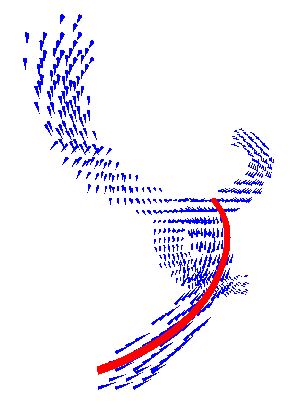
\includegraphics[width=72mm, height=100mm]{images/fibraecampo.png}
      \label{fig:fibraecampo}
      \caption{Campo 32x32x32 com duas hélices. Ao chegar na intersecção, a fibra se desvia para fora do campo e o método entende que terminou de propagá-la devido à baixa intensidade dos vetores.}
    \end{center}
  \end{figure}
  
  Indo além, os testes deste protótipo com ressonâncias reais gerou o mesmo resultado do software de exploração de imagens médicas BioImage Suite (\ref{bioimage}), como podemos observar a seguir.
  
  \begin{figure}[!h]
    \begin{center}
      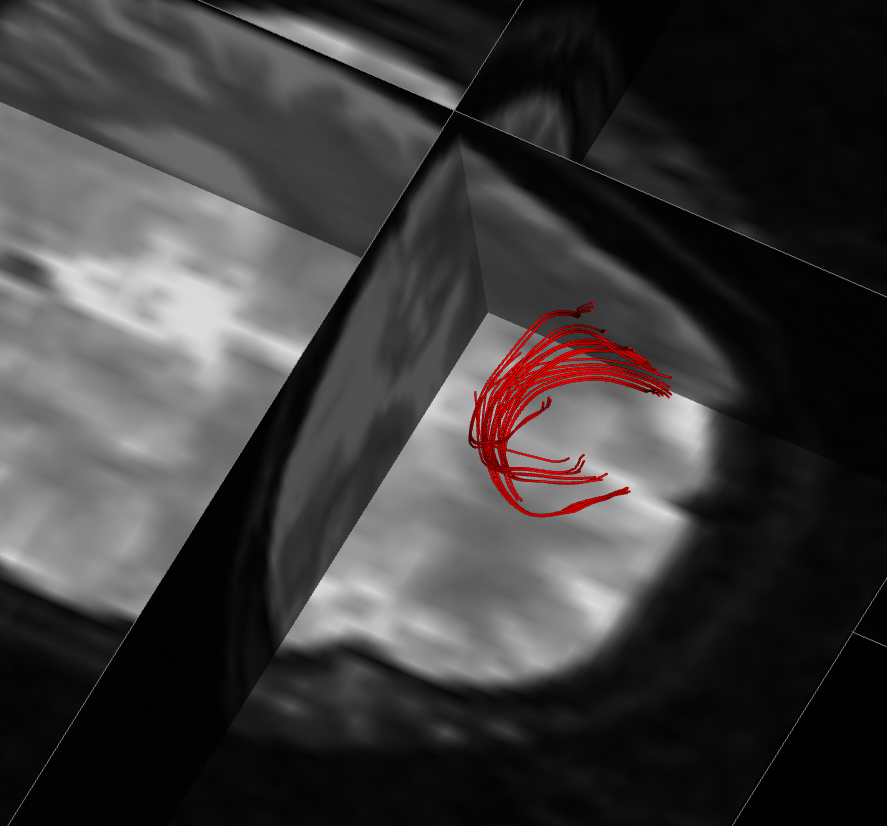
\includegraphics[width=100mm, height=72mm]{images/bioimage-dti.png}
      \label{fig:bioimage-dti}
      \caption{Resultado da tractografia realizada pelo BioImage Suite em uma ressonância magnética.}
    \end{center}
  \end{figure}
  
  \begin{figure}[!h]
    \begin{center}
      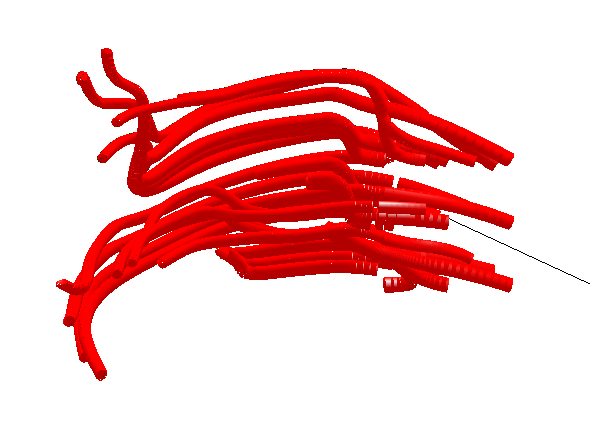
\includegraphics[width=100mm, height=72mm]{images/prototype-dti.png}
      \label{fig:prototype-dti}
      \caption{Resultado da tractografia realizada pelo pelo protótipo na mesma ressonância magnética da figura 4.2.}
    \end{center}
  \end{figure}
  
  Como podemos observar, o resultado (em vermelho) obtido por ambos é o mesmo, confirmando a corretude do protótipo gerado comparando-o a um software já consolidado.
  
  \subsection{Protótipo utilizando a VTK}
  Este protótipo utilizou a versão 5.6 da biblioteca \textit{VTK} para servir como uma prova de que é possível implementar o método dentro da biblioteca, posteriormente sendo útil para o planejamento do que deve ser feito para extende-lo em \textit{GPU} no futuro.
  
  A única dependência que existe, é a instalação da biblioteca \textit{VTK} 5.6. Com isto, sua compilação é ainda mais simples que o protótipo anterior utilizando software de compilação multiplataforma \textit{CMake}. Os resultados de uma compilação bem sucedida podem ser vistos a seguir:
  
  {\scriptsize
  \begin{verbatim}
  $ cmake .
  -- The C compiler identification is GNU 4.7.2
  -- The CXX compiler identification is GNU 4.7.2
  -- Check for working C compiler: /usr/bin/gcc
  -- Check for working C compiler: /usr/bin/gcc -- works
  -- Detecting C compiler ABI info
  -- Detecting C compiler ABI info - done
  -- Check for working CXX compiler: /usr/bin/c++
  -- Check for working CXX compiler: /usr/bin/c++ -- works
  -- Detecting CXX compiler ABI info
  -- Detecting CXX compiler ABI info - done
  -- Configuring done
  -- Generating done
  -- Build files have been written to: ./runge-kutta-vtk
  $ make
  Scanning dependencies of target RungeKutta
  [ 20%] Building CXX object CMakeFiles/RungeKutta.dir/Main.cpp.o
  [ 40%] Building CXX object CMakeFiles/RungeKutta.dir/io/input/Input.cpp.o
  [ 60%] Building CXX object CMakeFiles/RungeKutta.dir/io/input/AnalyzeReader.cpp.o
  [ 80%] Building CXX object CMakeFiles/RungeKutta.dir/core/cpp/Tracer.cpp.o
  [100%] Building CXX object CMakeFiles/RungeKutta.dir/io/output/Renderer.cpp.o
  Linking CXX executable RungeKutta
  [100%] Built target RungeKutta
  \end{verbatim}
  }
  
  Sua interface possui as mesmas funcionalidades que a do protótipo anterior, permitindo rotação, translação e escala. Da mesma forma este protótipo também não é capaz de lidar com indeterminações em um campo vetorial.
  
  \begin{figure}[!h]
    \begin{center}
      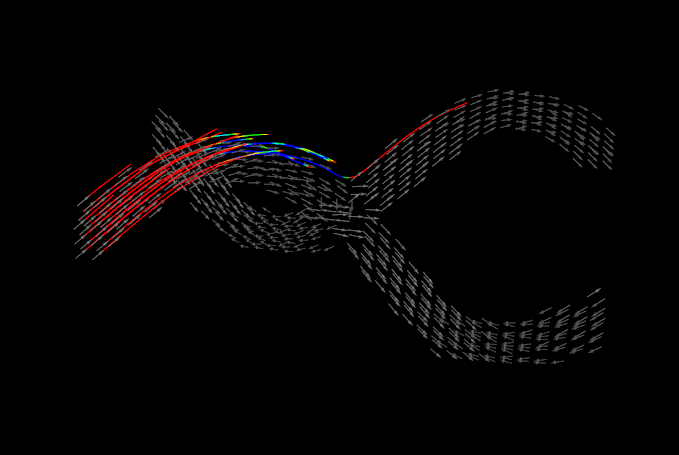
\includegraphics[width=100mm, height=72mm]{images/fibraecampo-vtk.png}
      \label{fig:fibraecampo-vtk}
      \caption{Campo 32x32x32 com duas hélices. Ao chegar na intersecção, a fibra se desvia para um fora do campo e o método entende que terminou de propaga-la devido à baixa intensidade dos vetores ou se desvia para outraq hélice devido à indeterminação do campo na intersecção.}
    \end{center}
  \end{figure}

\chapter{Conclusão}

\chapter{Referências Bibliográficas}

\section{Livros}
\begin{itemize}
  \item \label{numerical-recipes}PRESS, William H. et al. \textit{Numerical Recipes in C}
  \item \label{numerical-analysis}STOER, Josef; BULIRSCH, Roland. \textit{Introduction to Numerical Analysis}
\end{itemize}

\section{Artigos}
\begin{itemize}
  \item \label{fiber-tracking-article}Mori, S. and van Zijl, P. C. M. (2002), Fiber tracking: principles and strategies – a technical review. NMR Biomed., 15: 468–480. doi: 10.1002/nbm.781;
\end{itemize}

\section{Websites}
\subsection{Método de Integração Numérica de Runge-Kutta}
\begin{itemize}
  \item \href{http://math.fullerton.edu/mathews/n2003/Euler'sMethodMod.html}{\textit{Método de Euler - http://math.fullerton.edu/mathews/n2003/Euler'sMethodMod.html}} (acessado em 10/02/2012); 
  \item \href{http://apps.nrbook.com/c/index.html}{\textit{Numerical Recipes In C} - http://apps.nrbook.com/c/index.html} (acessado em 10/02/2012);
  \item \href{http://www.cmsoft.com.br/index.php?option=com_content&view=category&layout=blog&id=108&Itemid=162}{Solucionador de EDOs em OpenCL -\newline http://www.cmsoft.com.br/index.php?\newline option=com\_content\&view=category\&layout=blog\&id=108\&Itemid=162} (acessado em 26/02/2012).
\end{itemize}

\subsection{CUDA}
\begin{itemize}
  \item \href{http://developer.download.nvidia.com/compute/DevZone/docs/html/C/doc/CUDA_C_Programming_Guide.pdf}{Referência - http://developer.download.nvidia.com/compute/DevZone/docs/html/C/doc/\newline CUDA\_C\_Programming\_Guide.pdf} (acessado em 25/02/2012)
  \item \href{http://developer.download.nvidia.com/compute/DevZone/docs/html/C/doc/CUDA_C_Best_Practices_Guide.pdf}{Boas práticas - http://developer.download.nvidia.com/compute/DevZone/docs/html\newline/C/doc/CUDA\_C\_Best\_Practices\_Guide.pdf} (acessado em 25/02/2012)
\end{itemize}

\subsection{OpenCL}
\begin{itemize}
  \item \href{http://www.khronos.org/assets/uploads/developers/library/overview/opencl-overview.pdf}{http://www.khronos.org/assets/uploads/developers/library/overview/opencl-overview.pdf} (acessado em 26/02/2012);
  \item \href{http://developer.amd.com/zones/OpenCLZone/programming/Pages/default.aspx}{http://developer.amd.com/zones/OpenCLZone/programming/Pages/default.aspx} (acessado em 26/02/2012);
  \item \href{http://developer.download.nvidia.com/compute/cuda/3_2_prod/toolkit/docs/OpenCL_Programming_Guide.pdf}{http://developer.download.nvidia.com/compute/cuda/3\_2\_prod/toolkit/docs/\newline OpenCL\_Programming\_Guide.pdf} (acessado em  26/02/12);
  \item \href{http://developer.download.nvidia.com/compute/cuda/3_2_prod/toolkit/docs/OpenCL_Best_Practices_Guide.pdf}{http://developer.download.nvidia.com/compute/cuda/3\_2\_prod/toolkit/docs/\newline OpenCL\_Best\_Practices\_Guide.pdf} (acessado em 26/02/12);
  \item \href{http://www.khronos.org/opencl/}{http://www.khronos.org/opencl/} (acessado em 26/02/2012).
\end{itemize}

\subsection{OpenGL}
\begin{itemize}
  \item \href{https://github.com/curran/renderCyliner}{Conectar dois pontos com um cilindro - https://github.com/curran/renderCyliner} (acessado em 05/07/2012).
\end{itemize}

\subsection{Outros}
\begin{itemize}
  \item \label{medsquare}\href{http://ccsl.ime.usp.br/medsquare/}{MedSquare - http://ccsl.ime.usp.br/medsquare/}
  \item \label{gtx690}\href{http://www.nvidia.com.br/object/geforce-gtx-690-br.html}{Catálogo NVIDIA - http://www.nvidia.com.br/object/geforce-gtx-690-br.html}
\end{itemize}


\part{Subjetiva}
\chapter{Giancarlo Rigo}

\chapter{Rafael Reggiani Manzo}
Desenvolver este trabalho de conclusão de concurso foi fundamental para complementar minha formação como cientista da computação. Esta foi a primeira oportunidade de desenvolver um projeto durante todo um ano, com uma preocupação real com sua qualidade e interagindo com um docente frequentemente. Algo oposto aos trabalhos que usualmente são exigidos nas disciplinas onde eu trabalho neles durante no máximo um mês, com a preocupação de que o mínimo necessário esteja funcionando para o momento da correção e praticamente sem interagir com o professor.

Para alcançar este estado do trabalho, diversas disciplinas foram importantes e curiosamente duas delas são o Cálculo IV e a Álgebra Linear, que no momento quando cursei estas disciplinas jamais pensaria em utilizá-las. Estas duas disciplinas são toda a base matemática que foi necessária para ser possível reconstruir as trajetórias.

Igualmente importantes foram disciplinas básicas de computação como Princípios de Desenvolvimento de Algoritmos, onde pude ter o primeiro contato com conceitos como complexidade de algoritmos, estruturas de dados e até programação dinâmica.

Da mesma forma, na parte final do curso a disciplina de Computação Gráfica foi fundamental para tornar possível elaborar os protótipos que são o maior desta monografia.

Por fim, todas as disciplinas merecem o mérito por mostrarem, talvez não da melhor forma, como é possível aprender por conta própria o que é preciso para alcançar seu objetivo.


\end{document}
